\section{CCMP Agent Framework}
The ART testbed provides a base Agent class with several functions that must be
implemented by the new agent. These functions allow the agent to interact with
the other agents and participate in the game through the exchange of different
messages.  

To facilitate the distributed development environment it was important to break
the agent environment into different parts.  The CCMP Agent consists of the
base CCMP Agent class, base Trust Network interface class, a base Decision
Tree interface class and their associated implementations.

\subsection{Main Agent}
The base framework class, CCMPAgent, is the subclass of the ART testbed Agent
and provides the interface to the ART testbed.  The CCMPAgent is
responsible for handling the generation, parsing and responses to the
messages within the testbed Agent methods.  

It does this in a similar and abstract manner for each one. First it parses the
incoming messages and updates the trust network and decision tree on the
results of the messages, either positive or negative.  After updating the
knowledge base regarding the actions of the other agents and passing the new
values from the trust network to the decision tree, it queries the decision tree
to determine what action to take.  It then generates the appropriate
messages and passes them to the sim.

The base CCMPAgent class implements all this functionality in an abstract way
using the base TrustNetwork and DecisionTree classes.  The specific objects
types, such as the Bayesian trust network and Weka decision tree, are
instantiated in subclasses of CCMPAgent.  It is these subclasses that are passed
to the ART testbed for creation in the sim.  In this manner different
implementations of the trust network and decision tree classes can be easily
incorporated into the CCMPAgent.  The two derived classes developed for this 
project are shown in Figure~\ref{fig:CCMPClasses}.

\begin{figure}
\centering
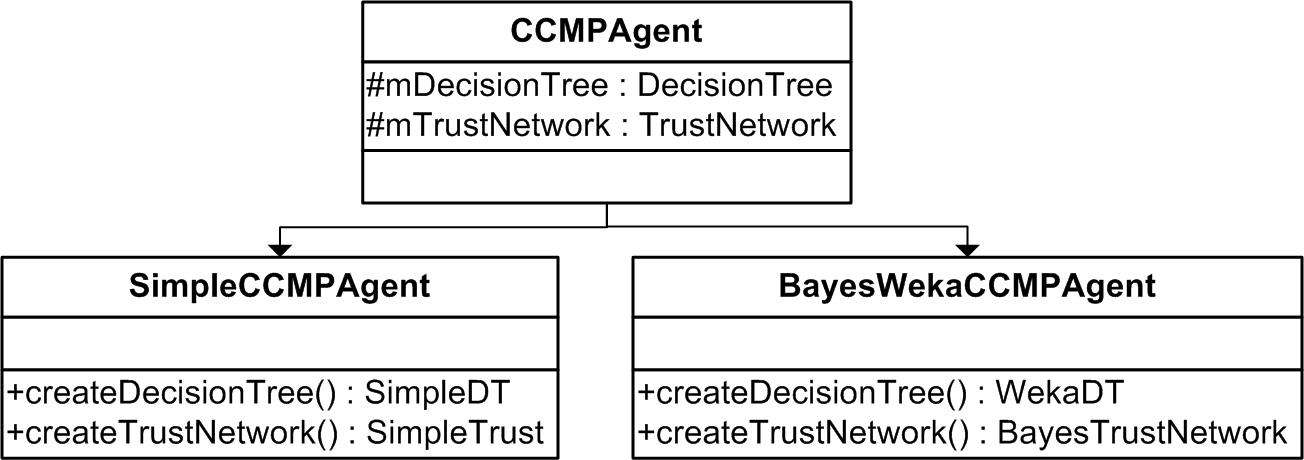
\includegraphics{images/CCMPClasses.jpg}
\caption{Extended Classes of the abstract CCMPAgent class.}
\label{fig:CCMPClasses}
\end{figure}

\subsection{Trust Network}
The trust network is an interface class used to represent the trust the agent
has for other players.  The interface class provides methods to update the
trust values based on events in the sim, such as receiving new reputation
information from other agents or negative actions taken by an agent.  During
each of the ART agent methods the CCMPAgent class will parse the incoming
messages to determine the actions of the other agents.  Based on these actions
and the contents of the messages the CCMPAgent will call the appropriate
function in the Trust Network to update the trust values.  At the end of each
frame the resulting final appraisal and each agents opinion are passed to the trust network 
to update the trust value for the agent based on the results. Table~\ref{table:TNUpdate}
shows the functions provided by the Trust Network to update the trust values.

\begin{table}[h]
\centering
\begin{tabular}{|l|l|}
\hline
\multicolumn{2}{|c|}{Reputation Updates} \\
\hline
receiveAgentReputationUpdate & updateAgentTrustFromFinalAppraisal \\
\hline
Actually provide a reputation response & Determine the reputation value to
return \\ 
\hline
\multicolumn{2}{|c|}{Negative Actions} \\
\hline
agentDidNotAcceptReputationRequest & agentDidNotProvideReputation \\
\hline
agentDidNotProvideCertainty & agentDidNotProvideOpinion \\
\hline
agentDidNotAcceptCertainty & \\
\hline
\end{tabular}
\caption{Agent Trust Network update functions.}
\label{table:TNUpdate}
\end{table}

The penalty values for the negative actions shown above have default values in the code,
but could be changed by setting the appropriate XML tag within the configuration XML file
of the agent.

\subsection{Decision Tree}
The decision tree interface class provides methods for the CCMP agent to
determine what actions to perform.  There are a finite number of actions, listed in Table~\ref{table:DTUpdate}
that an agent in the ART testbed can decide to perform.
\begin{table}[h]
\centering
\begin{tabular}{|l|l|}
\hline
\multicolumn{2}{|c|}{Reputation} \\
\hline
Ask another agent for a reputation & Accept another agents reputation request \\
\hline
Actually provide a reputation response & Determine the reputation value to
return \\ 
\hline
\multicolumn{2}{|c|}{Certainty} \\
\hline
Ask another agent for a certainty value & Accept another agents request for a
certainty \\
\hline
Actually provide a certainty response & Determine the certainty value to return
\\
\hline
\multicolumn{2}{|c|}{Opinions} \\
\hline
Ask another agent for an opinion & Accept another agents request for an
opinion \\
\hline
Actually generate the opinion & Determine the amount to pay for an
opinion \\
\hline
Modify the generated opinion & \\
\hline
\end{tabular}
\caption{Agent Decision Tree update functions.}
\label{table:DTUpdate}
\end{table}

As discussed above, during each of the ART agent methods the CCMPAgent class
will update the Trust Network, based on other agent actions, and then pass these
updated values to the Decision Tree.  The CCMPAgent then calls the appropriate
methods, shown in Table~\ref{table:DTUpdate}, in the Decision Tree interface class 
to get the actions to take for the particular method.  The CCMPAgent will also 
tell the Decision Tree about the negative actions of other agents, such as not 
providing a reputation after payment, as this may affect the actions recommended 
by the actual implementation class of the decision tree used by the agent.  
